\documentclass{article}
\usepackage[utf8]{inputenc}
\usepackage[margin=1in]{geometry}
\usepackage{lastpage}
\usepackage{fancyhdr}
\usepackage{tikz}
\usetikzlibrary{arrows}
\usepackage{multicol}
\usepackage{tabularx}
\usepackage{adjustbox}
\usepackage{color}
\usepackage{listings}
\usepackage{graphicx}
\usepackage{verbatim}
\usepackage{mathtools} 
\usepackage{amssymb}
\usepackage{amsmath}
\usepackage{algorithm}
\usepackage{algpseudocode}
\usepackage{url}
\usepackage{hyperref}

\pagestyle{fancy}
\lhead{Blaney}
\chead{\textit{Algorithm Analysis - Spring 2014}}
\rhead{Homework 1}
\cfoot{\thepage\ of \pageref{LastPage}}

\setlength{\parindent}{0pt}

\definecolor{mygreen}{rgb}{0,0.6,0}
\definecolor{mygray}{rgb}{0.5,0.5,0.5}
\definecolor{mymauve}{rgb}{0.58,0,0.82}

\lstset{ %
  backgroundcolor=\color{white},   % choose the background color; you must add \usepackage{color} or \usepackage{xcolor}
  basicstyle=\ttfamily\footnotesize,        % the size of the fonts that are used for the code
  breakatwhitespace=false,         % sets if automatic breaks should only happen at whitespace
  breaklines=true,                 % sets automatic line breaking
  captionpos=b,                    % sets the caption-position to bottom
  commentstyle=\color{mygreen},    % comment style
  deletekeywords={asdf,jkl},            % if you want to delete keywords from the given language
  escapeinside={\%*}{*)},          % if you want to add LaTeX within your code
  extendedchars=true,              % lets you use non-ASCII characters; for 8-bits encodings only, does not work with UTF-8
  frame=single,                    % adds a frame around the code
  keepspaces=true,                 % keeps spaces in text, useful for keeping indentation of code (possibly needs columns=flexible)
  keywordstyle=\color{blue},       % keyword style
  language=Python,                   % the language of the code
  morekeywords={var,function,window,document,console,undefined,Number,String,Boolean,Object,Array,Function,arguments,let,var},            % if you want to add more keywords to the set
  numbers=none,                    % where to put the line-numbers; possible values are (none, left, right)
  numbersep=5pt,                   % how far the line-numbers are from the code
  numberstyle=\tiny\color{mygray}, % the style that is used for the line-numbers
  rulecolor=\color{black},         % if not set, the frame-color may be changed on line-breaks within not-black text (e.g. comments (green here))
  showspaces=false,                % show spaces everywhere adding particular underscores; it overrides 'showstringspaces'
  showstringspaces=false,          % underline spaces within strings only
  showtabs=false,                  % show tabs within strings adding particular underscores
  stepnumber=1,                    % the step between two line-numbers. If it's 1, each line will be numbered
  stringstyle=\color{mymauve},     % string literal style
  tabsize=2,                       % sets default tabsize to 2 spaces
}

\title{CS319}
\author{Jim Blaney}
\date{January 2014}

\begin{document}

\noindent I pledge that I have neither given nor received any unauthorized aid on this assignment. \\[4em]
%\-\hspace{0.55\linewidth} \includegraphics[height=4em]{signature-latex}

\section*{Problem 1 [PART COMPLETE-TIME]}

\begin{enumerate}
  \item[i.] \url{http://www.proofwiki.org/wiki/Sum_of_Geometric_Progression#Proof_1}
  \item[ii.] \url{http://www.proofwiki.org/wiki/Sum_of_Sequence_of_Squares#Proof_1}
\end{enumerate}

\section*{Problem 2 [COMPLETE]}

\subsection*{Solutions}
  \begin{multicols}{2}
    \subsubsection*{Iterative Solution}
      \lstinputlisting{02-iterative.py}
    \subsubsection*{Recursive Solution}
      \lstinputlisting{02-recursive.py}
  \end{multicols}

\subsection*{Results}

\begin{minipage}{.57\linewidth}
  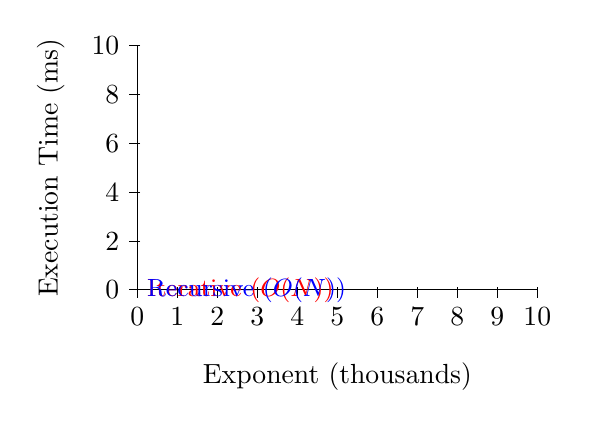
\begin{tikzpicture}[y=.31cm, x=.2in]
    %axis
    \draw (0,0) -- coordinate (x axis mid) (10,0);
    \draw (0,0) -- coordinate (y axis mid) (0,10);
    
    %ticks
    \foreach \x in {0,1,...,10}
        \draw (\x,1pt) -- (\x,-3pt) node[anchor=north] {\x};
    \foreach \y in {0,2,...,10}
        \draw (1pt,\y) -- (-3pt,\y) node[anchor=east] {\y}; 
        
    %labels      
    \node[below=0.8cm] at (x axis mid) {Exponent (thousands)};
    \node[rotate=90, above=0.8cm] at (y axis mid) {Execution Time (ms)};

    %plots
    \draw[color=red] plot[id=iterative] file {02-results-iterative.data} node[right] {\small Iterative ($O(N)$)};
    \draw[color=blue] plot[id=recursive] file {02-results-recursive.data} node[right] {\small Recursive ($O(N)$)};
    
\end{tikzpicture}
\end{minipage}
\begin{minipage}{.43\linewidth}
  \begin{tabularx}{\textwidth}{c||c|c}
Exponent  &  Iterative (ms) &  Recursive (ms) \\
\hline
0      &  0.003099  &  0.000954 \\
1000   &  0.155926  &  0.432014 \\
2000   &  0.421047  &  1.115080 \\
3000   &  0.810862  &  1.724000 \\
4000   &  1.162050  &  2.570150 \\
5000   &  1.710890  &  3.561020 \\
6000   &  2.199890  &  4.256960 \\
7000   &  3.059150  &  5.470040 \\
8000   &  3.557920  &  6.670000 \\
9000   &  4.281040  &  7.956980 \\
10000  &  5.115030  &  9.102110 \\
\end{tabularx}
\end{minipage}

\subsection*{Findings}

The iterative function has to iterate over the range of the exponent a single time ($n$), while the number of iterations of the recursive function is calculated by the function $a_1 = 1, a_n = 1 + a_{n - 1}$. The iterative function has a growth function of $O(N)$, and the recursive function also has a growth of $O(N)$. The iterative function operates more efficiently than the recursive function because, in the recursive function, the application runtime has to push arguments and addresses to the call stack and invoke itself $n - 1$ times in order to calculate the value. In the iterative solution, this happens $1$ time.

\section*{Problem 3 [COMPLETE]}


\adjustbox{valign=t}{
\begin{minipage}[t]{.33\linewidth}
  1. \textit{insert(10)} \\[1em]
  \adjustbox{valign=t}{
    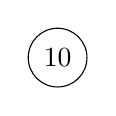
\begin{tikzpicture}[->,>=latex]
      \node[circle,draw](z){$10$};
    \end{tikzpicture}
  }
\end{minipage}  
}
\adjustbox{valign=t}{
\begin{minipage}[t]{.33\linewidth}
2. \textit{insert(5)} \\[1em]
  \adjustbox{valign=t}{
    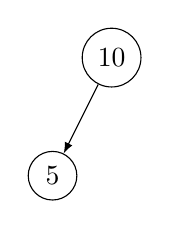
\begin{tikzpicture}[->,>=latex]
      \node[circle,draw](z){$10$}
        child{
          node[circle,draw]{$5$}
        }
        child[missing]{};
    \end{tikzpicture}
  }
\end{minipage}  
}
\adjustbox{valign=t}{
\begin{minipage}[t]{.33\linewidth}
  3. \textit{insert(15)} \\[1em]
  \adjustbox{valign=t}{
    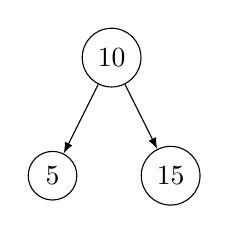
\begin{tikzpicture}[->,>=latex]
      \node[circle,draw](z){$10$}
        child{
          node[circle,draw]{$5$}
        }
        child{
          node[circle,draw]{$15$}
        };
    \end{tikzpicture}
  }
\end{minipage}
} \\[2em]
\adjustbox{valign=t}{
\begin{minipage}[t]{.33\linewidth}  
  4. \textit{insert(10)} \\[1em]
  \adjustbox{valign=t}{
    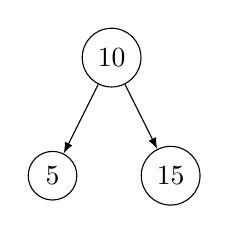
\begin{tikzpicture}[->,>=latex]
      \node[circle,draw](z){$10$}
        child{
          node[circle,draw]{$5$}
        }
        child{
          node[circle,draw]{$15$}
        };
    \end{tikzpicture}
  }
\end{minipage}  
}
\adjustbox{valign=t}{
\begin{minipage}{.33\linewidth}
  5. \textit{insert(9)} \\[1em]
  \adjustbox{valign=t}{
    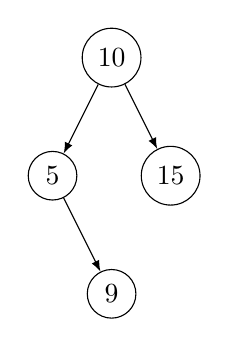
\begin{tikzpicture}[->,>=latex]
      \node[circle,draw](z){$10$}
        child{
          node[circle,draw]{$5$}
          child[missing]{}
          child {
            node[circle,draw]{$9$}
          }
        }
        child{
          node[circle,draw]{$15$}
        };
    \end{tikzpicture}
  }
\end{minipage}  
}
\adjustbox{valign=t}{
\begin{minipage}{.33\linewidth}
  6. \textit{insert(7)} \\[1em]
  \adjustbox{valign=t}{
    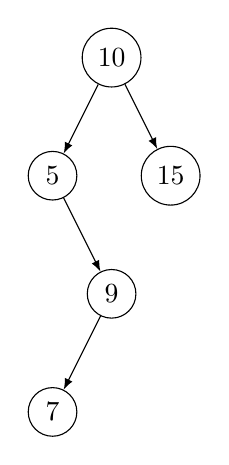
\begin{tikzpicture}[->,>=latex]
      \node[circle,draw](z){$10$}
        child{
          node[circle,draw]{$5$}
          child[missing]{}
          child {
            node[circle,draw]{$9$}
            child {
              node[circle,draw]{$7$}
            }
            child[missing]{}
          }
        }
        child{
          node[circle,draw]{$15$}
        };
    \end{tikzpicture}
  }\end{minipage}  
} \\[2em]
\adjustbox{valign=t}{
\begin{minipage}{.33\linewidth}
  7. \textit{insert(2)} \\[1em]
  \adjustbox{valign=t}{
    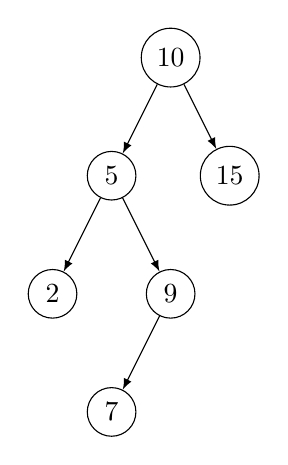
\begin{tikzpicture}[->,>=latex]
      \node[circle,draw](z){$10$}
        child{
          node[circle,draw]{$5$}
          child {
            node[circle,draw]{$2$}
          }
          child {
            node[circle,draw]{$9$}
            child {
              node[circle,draw]{$7$}
            }
            child[missing]{}
          }
        }
        child{
          node[circle,draw]{$15$}
        };
    \end{tikzpicture}
  }
\end{minipage}  
}
\adjustbox{valign=t}{
\begin{minipage}{.33\linewidth}
  8. \textit{insert(1)} \\[1em]
  \adjustbox{valign=t}{
    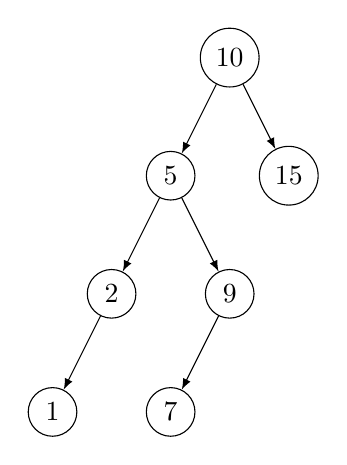
\begin{tikzpicture}[->,>=latex]
      \node[circle,draw](z){$10$}
        child{
          node[circle,draw]{$5$}
          child {
            node[circle,draw]{$2$}
            child {
              node[circle,draw]{$1$}
            }
            child[missing] { }
          }
          child {
            node[circle,draw]{$9$}
            child {
              node[circle,draw]{$7$}
            }
            child[missing]{}
          }
        }
        child{
          node[circle,draw]{$15$}
        };
    \end{tikzpicture}
  }
\end{minipage}  
}
\adjustbox{valign=t}{
\begin{minipage}{.33\linewidth}
  9. \textit{insert(4)} \\[1em]
  \adjustbox{valign=t}{
    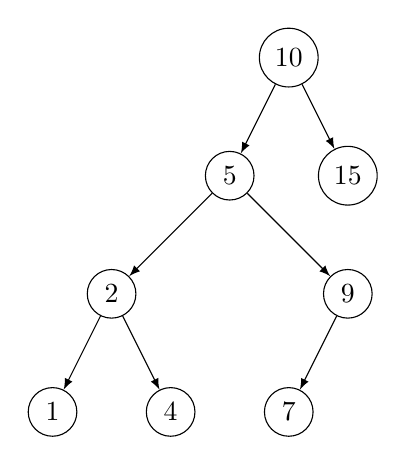
\begin{tikzpicture}[->,>=latex]
      \node[circle,draw](z){$10$}
        child{
          node[circle,draw]{$5$}
          child {
            node[circle,draw]{$2$}
            child {
              node[circle,draw]{$1$}
            }
            child {
              node[circle,draw]{$4$}
            }
          }
          child[missing]
          child {
            node[circle,draw]{$9$}
            child {
              node[circle,draw]{$7$}
            }
            child[missing]{}
          }
        }
        child{
          node[circle,draw]{$15$}
        };
    \end{tikzpicture}
  }
\end{minipage}  
} \\[2em]
\adjustbox{valign=t}{
\begin{minipage}{.33\linewidth}
  10. \textit{insert(3)} \\[1em]
  \adjustbox{valign=t}{
    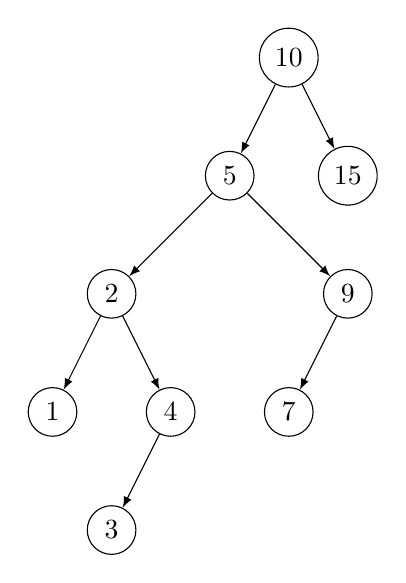
\begin{tikzpicture}[->,>=latex]
      \node[circle,draw](z){$10$}
        child{
          node[circle,draw]{$5$}
          child {
            node[circle,draw]{$2$}
            child {
              node[circle,draw]{$1$}
            }
            child {
              node[circle,draw]{$4$}
              child {
                node[circle,draw]{$3$}
              }
              child[missing] { }
            }
          }
          child[missing]
          child {
            node[circle,draw]{$9$}
            child {
              node[circle,draw]{$7$}
            }
            child[missing]{}
          }
        }
        child{
          node[circle,draw]{$15$}
        };
    \end{tikzpicture}
  }
\end{minipage}  
}
\adjustbox{valign=t}{
\begin{minipage}{.33\linewidth}
  11. \textit{insert(8)} \\[1em]
  \adjustbox{valign=t}{
    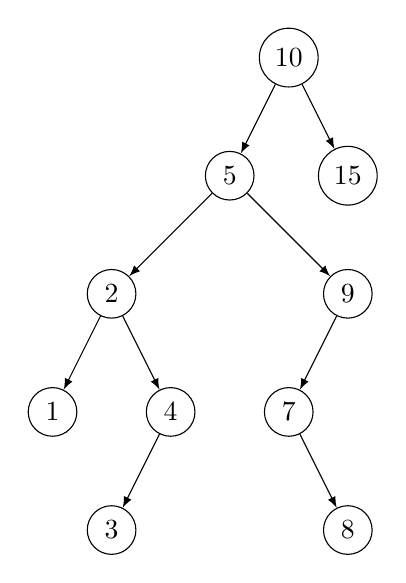
\begin{tikzpicture}[->,>=latex]
      \node[circle,draw](z){$10$}
        child{
          node[circle,draw]{$5$}
          child {
            node[circle,draw]{$2$}
            child {
              node[circle,draw]{$1$}
            }
            child {
              node[circle,draw]{$4$}
              child {
                node[circle,draw]{$3$}
              }
              child[missing]{ }
            }
          }
          child[missing]
          child {
            node[circle,draw]{$9$}
            child {
              node[circle,draw]{$7$}
              child[missing]{ }
              child {
                node[circle,draw]{$8$}
              }
            }
            child[missing]{}
          }
        }
        child{
          node[circle,draw]{$15$}
        };
    \end{tikzpicture}
  }
\end{minipage}  
}
\adjustbox{valign=t}{
\begin{minipage}{.33\linewidth}
  12. \textit{delete(5)} \\[1em]
  \adjustbox{valign=t}{
    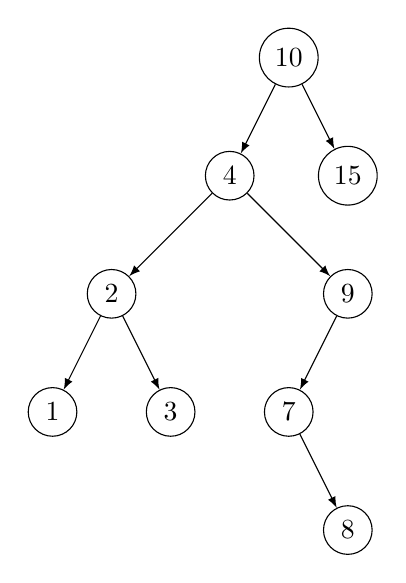
\begin{tikzpicture}[->,>=latex]
      \node[circle,draw](z){$10$}
        child{
          node[circle,draw]{$4$}
          child {
            node[circle,draw]{$2$}
            child {
              node[circle,draw]{$1$}
            }
            child {
              node[circle,draw]{$3$}
            }
          }
          child[missing]
          child {
            node[circle,draw]{$9$}
            child {
              node[circle,draw]{$7$}
              child[missing]{ }
              child {
                node[circle,draw]{$8$}
              }
            }
            child[missing]{}
          }
        }
        child{
          node[circle,draw]{$15$}
        };
    \end{tikzpicture}
  }
\end{minipage}  
}


\section*{Problem 4 [COMPLETE]}

\begin{enumerate}
  \item[(a)] 
\adjustbox{valign=t}{
\begin{minipage}[t]{.33\linewidth}
  1. \textit{insert(18)} \\[1em]
  \adjustbox{valign=t}{
    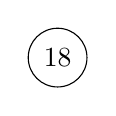
\begin{tikzpicture}
      \node[circle,draw](z){$18$};
    \end{tikzpicture}
  }
\end{minipage}  
}
\adjustbox{valign=t}{
\begin{minipage}[t]{.33\linewidth}
  2. \textit{insert(10)} \\[1em]
  \adjustbox{valign=t}{
    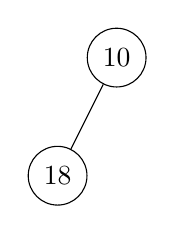
\begin{tikzpicture}
      \node[circle,draw](z){$10$}
        child{
          node[circle,draw]{$18$}
        }
        child[missing]{};
    \end{tikzpicture}
  }
\end{minipage}  
}
\adjustbox{valign=t}{
\begin{minipage}[t]{.33\linewidth}
  3. \textit{insert(14)} \\[1em]
  \adjustbox{valign=t}{
    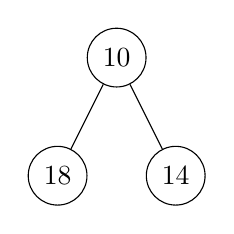
\begin{tikzpicture}
      \node[circle,draw](z){$10$}
        child{
          node[circle,draw]{$18$}
        }
        child{
          node[circle,draw]{$14$}
        };
    \end{tikzpicture}
  }
\end{minipage}  
} \\[2em]

\adjustbox{valign=t}{
\begin{minipage}[t]{.33\linewidth}
  4. \textit{insert(9)} \\[1em]
  \adjustbox{valign=t}{
    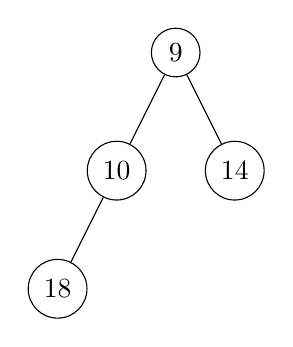
\begin{tikzpicture}
      \node[circle,draw](z){$9$}
        child{
          node[circle,draw]{$10$}
          child {
            node[circle,draw]{$18$}
          }
          child[missing] { }
        }
        child{
          node[circle,draw]{$14$}
        };
    \end{tikzpicture}
  }
\end{minipage}  
}
\adjustbox{valign=t}{
\begin{minipage}[t]{.33\linewidth}
  5. \textit{insert(2)} \\[1em]
  \adjustbox{valign=t}{
    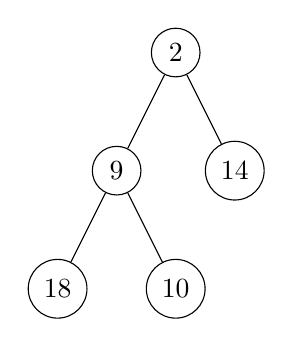
\begin{tikzpicture}
      \node[circle,draw](z){$2$}
        child{
          node[circle,draw]{$9$}
          child {
            node[circle,draw]{$18$}
          }
          child {
            node[circle,draw]{$10$}
          }
        }
        child{
          node[circle,draw]{$14$}
        };
    \end{tikzpicture}
  }
\end{minipage}  
} 
\adjustbox{valign=t}{
\begin{minipage}[t]{.33\linewidth}
  6. \textit{insert(7)} \\[1em]
  \adjustbox{valign=t}{
    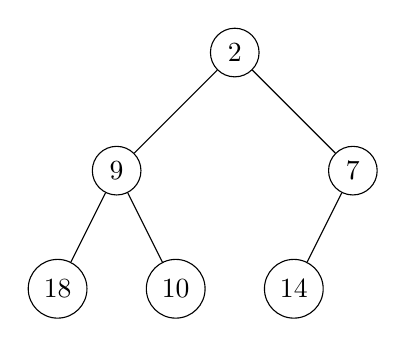
\begin{tikzpicture}
      \node[circle,draw](z){$2$}
        child{
          node[circle,draw]{$9$}
          child {
            node[circle,draw]{$18$}
          }
          child {
            node[circle,draw]{$10$}
          }
        }
        child[missing] { }
        child{
          node[circle,draw]{$7$}
          child {
            node[circle,draw]{$14$}
          }
          child[missing] { }
        };
    \end{tikzpicture}
  }
\end{minipage}  
} \\[2em]

\adjustbox{valign=t}{
\begin{minipage}[t]{.5\linewidth}
  7. \textit{insert(11)} \\[1em]
  \adjustbox{valign=t}{
    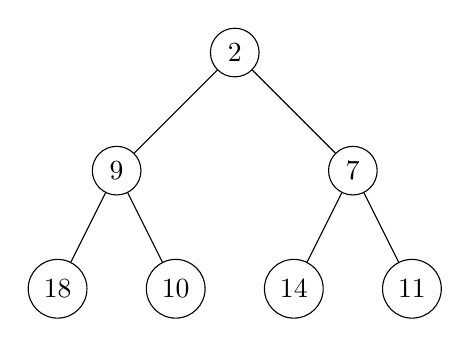
\begin{tikzpicture}
      \node[circle,draw](z){$2$}
        child{
          node[circle,draw]{$9$}
          child {
            node[circle,draw]{$18$}
          }
          child {
            node[circle,draw]{$10$}
          }
        }
        child[missing] { }
        child{
          node[circle,draw]{$7$}
          child {
            node[circle,draw]{$14$}
          }
          child {
            node[circle,draw]{$11$}
          }
        };
    \end{tikzpicture}
  }
\end{minipage}  
}
\adjustbox{valign=t}{
\begin{minipage}[t]{.5\linewidth}
  8. \textit{insert(12)} \\[1em]
  \adjustbox{valign=t}{
    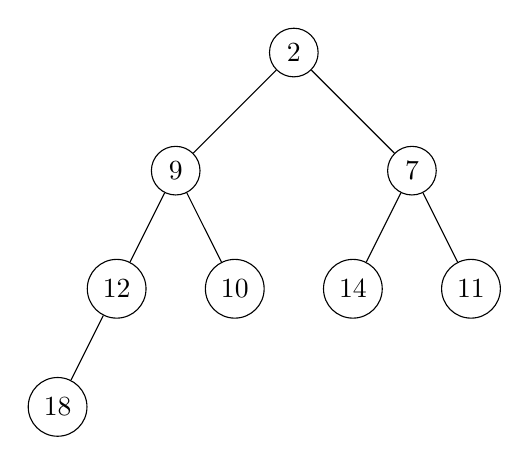
\begin{tikzpicture}
      \node[circle,draw](z){$2$}
        child{
          node[circle,draw]{$9$}
          child {
            node[circle,draw]{$12$}
            child { 
              node[circle,draw]{$18$}
            }
            child[missing] { }
          }
          child {
            node[circle,draw]{$10$}
          }
        }
        child[missing] { }
        child{
          node[circle,draw]{$7$}
          child {
            node[circle,draw]{$14$}
          }
          child {
            node[circle,draw]{$11$}
          }
        };
    \end{tikzpicture}
  }
\end{minipage}  
} \\[2em]

\adjustbox{valign=t}{
\begin{minipage}[t]{.5\linewidth}
  9. \textit{delete-top()} \\[1em]
  \adjustbox{valign=t}{
    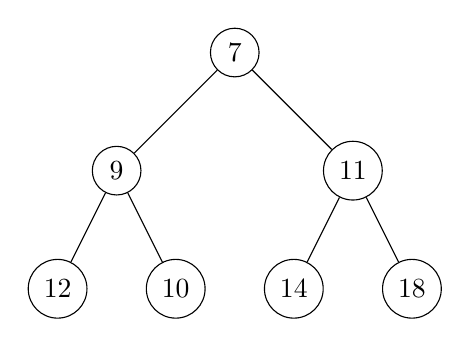
\begin{tikzpicture}
      \node[circle,draw](z){$7$}
        child{
          node[circle,draw]{$9$}
          child {
            node[circle,draw]{$12$}
          }
          child {
            node[circle,draw]{$10$}
          }
        }
        child[missing] { }
        child{
          node[circle,draw]{$11$}
          child {
            node[circle,draw]{$14$}
          }
          child {
            node[circle,draw]{$18$}
          }
        };
    \end{tikzpicture}
  }
\end{minipage}
} \\[2em]
  \item[(b)] \adjustbox{valign=t}{
\begin{minipage}[t]{.5\linewidth}
  1. \textit{min-heap} \\[1em]
  \adjustbox{valign=t}{
    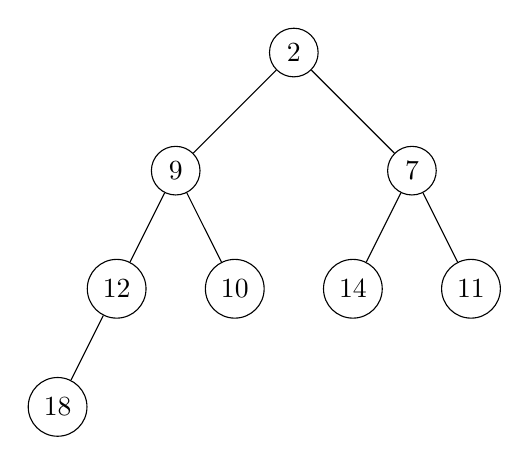
\begin{tikzpicture}
      \node[circle,draw](z){$2$}
        child{
          node[circle,draw]{$9$}
          child {
            node[circle,draw]{$12$}
            child { 
              node[circle,draw]{$18$}
            }
            child[missing] { }
          }
          child {
            node[circle,draw]{$10$}
          }
        }
        child[missing] { }
        child{
          node[circle,draw]{$7$}
          child {
            node[circle,draw]{$14$}
          }
          child {
            node[circle,draw]{$11$}
          }
        };
    \end{tikzpicture}
  }
\end{minipage}
}
\adjustbox{valign=t}{
\begin{minipage}[t]{.5\linewidth}
  2. \textit{Step 1} \\[1em]
  \adjustbox{valign=t}{
    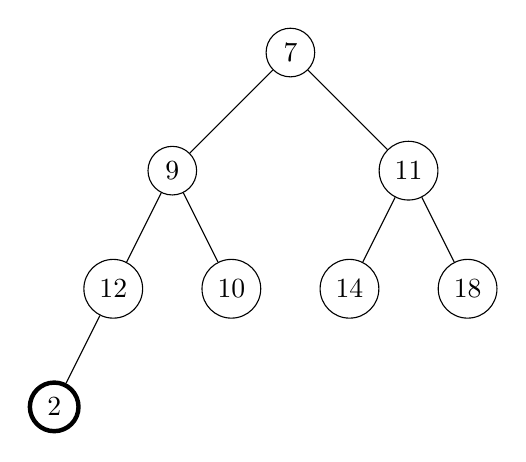
\begin{tikzpicture}
      \node[circle,draw](z){$7$}
        child{
          node[circle,draw]{$9$}
          child {
            node[circle,draw]{$12$}
            child { 
              node[circle,line width=1.6pt,draw]{$2$}
            }
            child[missing] { }
          }
          child {
            node[circle,draw]{$10$}
          }
        }
        child[missing] { }
        child{
          node[circle,draw]{$11$}
          child {
            node[circle,draw]{$14$}
          }
          child {
            node[circle,draw]{$18$}
          }
        };
    \end{tikzpicture}
  }
\end{minipage}
} \\[2em]

\adjustbox{valign=t}{
\begin{minipage}[t]{.5\linewidth}
  3. \textit{Step 2} \\[1em]
  \adjustbox{valign=t}{
    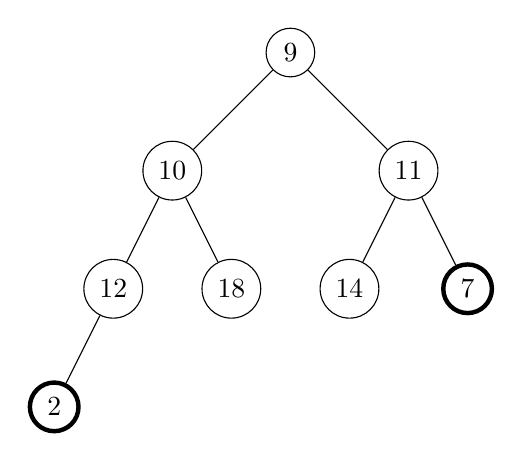
\begin{tikzpicture}
      \node[circle,draw](z){$9$}
        child{
          node[circle,draw]{$10$}
          child {
            node[circle,draw]{$12$}
            child { 
              node[circle,line width=1.6pt,draw]{$2$}
            }
            child[missing] { }
          }
          child {
            node[circle,draw]{$18$}
          }
        }
        child[missing] { }
        child{
          node[circle,draw]{$11$}
          child {
            node[circle,draw]{$14$}
          }
          child {
            node[circle,line width=1.6pt,draw]{$7$}
          }
        };
    \end{tikzpicture}
  }
\end{minipage}
}
\adjustbox{valign=t}{
\begin{minipage}[t]{.5\linewidth}
  4. \textit{Step 3} \\[1em]
  \adjustbox{valign=t}{
    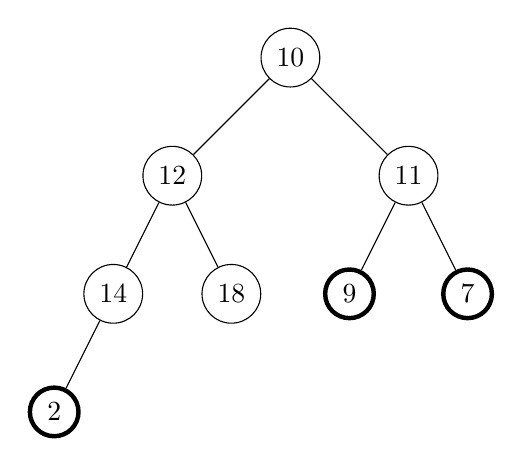
\begin{tikzpicture}
      \node[circle,draw](z){$10$}
        child{
          node[circle,draw]{$12$}
          child {
            node[circle,draw]{$14$}
            child { 
              node[circle,line width=1.6pt,draw]{$2$}
            }
            child[missing] { }
          }
          child {
            node[circle,draw]{$18$}
          }
        }
        child[missing] { }
        child{
          node[circle,draw]{$11$}
          child {
            node[circle,line width=1.6pt,draw]{$9$}
          }
          child {
            node[circle,line width=1.6pt,draw]{$7$}
          }
        };
    \end{tikzpicture}
  }
\end{minipage}
} \\[2em]

\adjustbox{valign=t}{
\begin{minipage}[t]{.5\linewidth}
  5. \textit{Step 4} \\[1em]
  \adjustbox{valign=t}{
    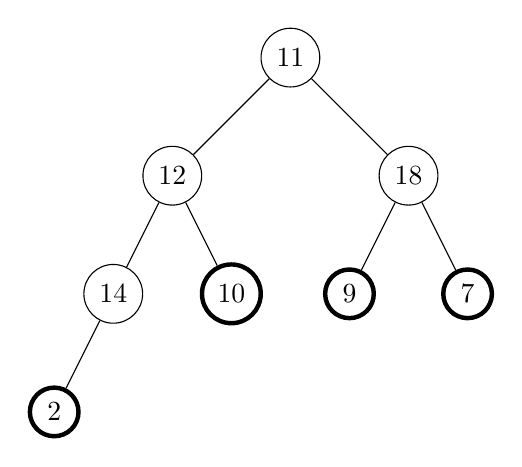
\begin{tikzpicture}
      \node[circle,draw](z){$11$}
        child{
          node[circle,draw]{$12$}
          child {
            node[circle,draw]{$14$}
            child { 
              node[circle,line width=1.6pt,draw]{$2$}
            }
            child[missing] { }
          }
          child {
            node[circle,line width=1.6pt,draw]{$10$}
          }
        }
        child[missing] { }
        child{
          node[circle,draw]{$18$}
          child {
            node[circle,line width=1.6pt,draw]{$9$}
          }
          child {
            node[circle,line width=1.6pt,draw]{$7$}
          }
        };
    \end{tikzpicture}
  }
\end{minipage}
}
\adjustbox{valign=t}{
\begin{minipage}[t]{.5\linewidth}
  6. \textit{Step 5} \\[1em]
  \adjustbox{valign=t}{
    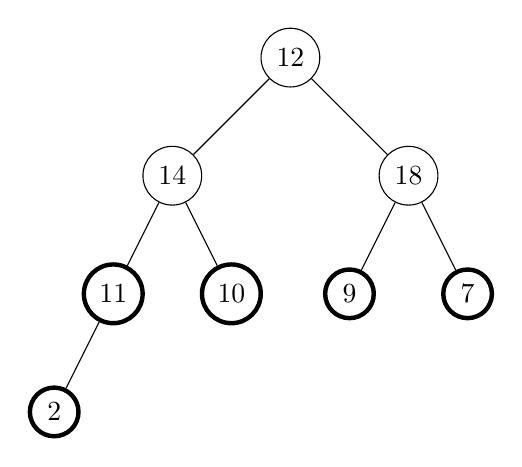
\begin{tikzpicture}
      \node[circle,draw](z){$12$}
        child{
          node[circle,draw]{$14$}
          child {
            node[circle,line width=1.6pt,draw]{$11$}
            child { 
              node[circle,line width=1.6pt,draw]{$2$}
            }
            child[missing] { }
          }
          child {
            node[circle,line width=1.6pt,draw]{$10$}
          }
        }
        child[missing] { }
        child{
          node[circle,draw]{$18$}
          child {
            node[circle,line width=1.6pt,draw]{$9$}
          }
          child {
            node[circle,line width=1.6pt,draw]{$7$}
          }
        };
    \end{tikzpicture}
  }
\end{minipage}
} \\[2em]

\adjustbox{valign=t}{
\begin{minipage}[t]{.5\linewidth}
  7. \textit{Step 6} \\[1em]
  \adjustbox{valign=t}{
    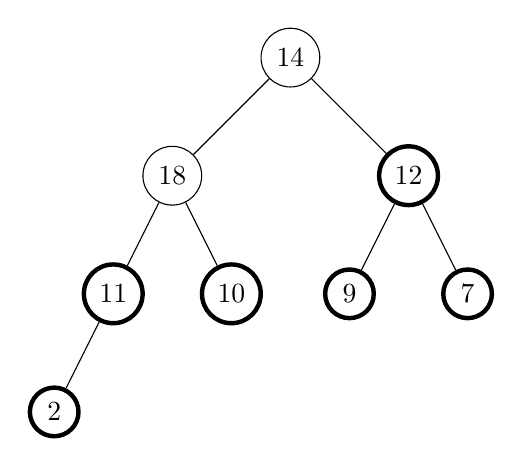
\begin{tikzpicture}
      \node[circle,draw](z){$14$}
        child{
          node[circle,draw]{$18$}
          child {
            node[circle,line width=1.6pt,draw]{$11$}
            child { 
              node[circle,line width=1.6pt,draw]{$2$}
            }
            child[missing] { }
          }
          child {
            node[circle,line width=1.6pt,draw]{$10$}
          }
        }
        child[missing] { }
        child{
          node[circle,line width=1.6pt,draw]{$12$}
          child {
            node[circle,line width=1.6pt,draw]{$9$}
          }
          child {
            node[circle,line width=1.6pt,draw]{$7$}
          }
        };
    \end{tikzpicture}
  }
\end{minipage}
}
\adjustbox{valign=t}{
\begin{minipage}[t]{.5\linewidth}
  8. \textit{Step 7} \\[1em]
  \adjustbox{valign=t}{
    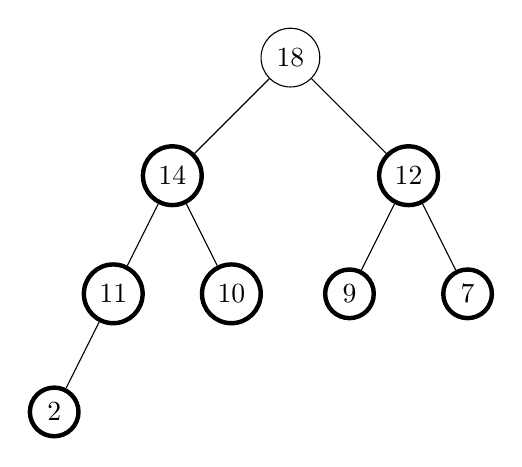
\begin{tikzpicture}
      \node[circle,draw](z){$18$}
        child{
          node[circle,line width=1.6pt,draw]{$14$}
          child {
            node[circle,line width=1.6pt,draw]{$11$}
            child { 
              node[circle,line width=1.6pt,draw]{$2$}
            }
            child[missing] { }
          }
          child {
            node[circle,line width=1.6pt,draw]{$10$}
          }
        }
        child[missing] { }
        child{
          node[circle,line width=1.6pt,draw]{$12$}
          child {
            node[circle,line width=1.6pt,draw]{$9$}
          }
          child {
            node[circle,line width=1.6pt,draw]{$7$}
          }
        };
    \end{tikzpicture}
  }
\end{minipage}
} \\[2em]

\adjustbox{valign=t}{
\begin{minipage}[t]{.5\linewidth}
  9. \textit{Step 8 (sorted)} \\[1em]
  \adjustbox{valign=t}{
    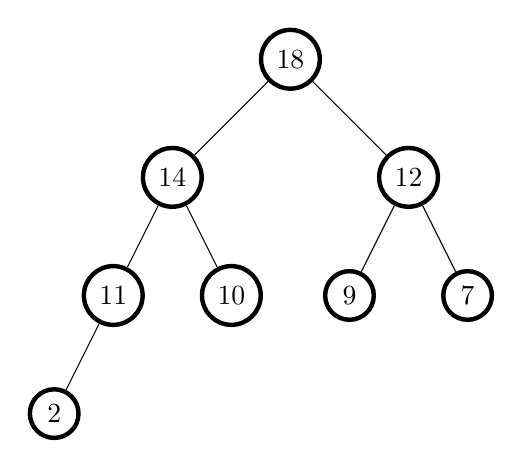
\begin{tikzpicture}
      \node[circle,line width=1.6pt,draw](z){$18$}
        child{
          node[circle,line width=1.6pt,draw]{$14$}
          child {
            node[circle,line width=1.6pt,draw]{$11$}
            child { 
              node[circle,line width=1.6pt,draw]{$2$}
            }
            child[missing] { }
          }
          child {
            node[circle,line width=1.6pt,draw]{$10$}
          }
        }
        child[missing] { }
        child{
          node[circle,line width=1.6pt,draw]{$12$}
          child {
            node[circle,line width=1.6pt,draw]{$9$}
          }
          child {
            node[circle,line width=1.6pt,draw]{$7$}
          }
        };
    \end{tikzpicture}
  }
\end{minipage}
} \\
\end{enumerate}

\section*{Problem 5 [COMPLETE]}

\begin{algorithm}[H]
\caption{Computes the number of leaves in a binary tree}
\textbf{Inputs:} $T$, a binary tree \\
\textbf{Outputs:} The number of leaf nodes in the initially-provided binary tree \\
\textbf{Complexity:} $O(N)$. Each node is computed against one time
\hline
\begin{algorithmic}[1]
  \Function{CountLeaves}{$T$}
    \If {$T = null $}
      \State \Return {$0$}
    \ElsIf {$T.left = null \And T.right = null$}
      \State \Return{$1$}
    \Else
      \State \Return \Call{CountLeaves}{$T.left$} $+$ \Call{CountLeaves}{$T.right$} 
    \EndIf
  \EndFunction
\end{algorithmic}
\end{algorithm}

\begin{algorithm}[H]
\caption{Computes the height of a node in a binary tree}
\textbf{Inputs:} $T$, a binary tree \\
\textbf{Outputs:} The height of the initally-provided binary tree \\
\textbf{Complexity:} $O(N)$. Each node is computed against one time
\hline
\begin{algorithmic}[1]
  \Function{NodeHeight}{$T$}
    \If {$T = null$}
      \State \Return {$0$}
    \EndIf
    \State $leftHeight :=$ \Call{NodeHeight}{$T.left$}
    \State $rightHeight :=$ \Call{NodeHeight}{$T.right$}
    \State \Return $1\ +$ \Call{Max}{$leftHeight$, $rightHeight$}
  \EndFunction
\end{algorithmic}
\end{algorithm}

\begin{algorithm}[H]
\caption{Computes the maximum depth of a binary tree}
\textbf{Inputs:} $T$, a binary tree \\
\textbf{Outputs:} The maximum depth of the initally-provided binary tree from the root node to the farthest leaf \\
\textbf{Complexity:} $O(log(N))$. Each node is computed against its parent one time, reducing the number of computations (compared to $N$) by half for each iteration
\hline
\begin{algorithmic}[1]
  \Function{NodeDepth}{$T$}
    \If {$T.parent = null$}
      \State \Return {$0$}
    \Else
      \State \Return $1\ +$ \Call{NodeDepth}{$T.Parent$}
    \EndIf
  \EndFunction
\end{algorithmic}
\end{algorithm}

\begin{algorithm}[H]
\caption{Indicates whether a binary tree is full (or not)}
\textbf{Inputs:} $T$, a binary tree \\
\textbf{Outputs:} The state of fullnes of the initially-provided binary tree \\
\textbf{Complexity:} $O(N)$. Each node is computed against one time
\hline
\begin{algorithmic}[1]
  \Function{IsFull}{$T$}
    \If {$T.left \not= null \And T.right \not= null$} %\Comment{The node has both children}
      \State \Return{\Call{IsFull}{$T.left$} $\And$ \Call{IsFull}{$T.right$}}
    \ElsIf {$T.left = null \And T.right = null$} %\Comment{The node is a leaf}
      \State \Return{$true$}
    \Else %\Comment{The node is not full}
      \State \Return{$false$}
    \EndIf
  \EndFunction
\end{algorithmic}
\end{algorithm}


\section*{Problem 6 [COMPLETE]}

The worst time complexity to compute the sum of a $n \times n$ 2-dimensional array is $O(N^2)$, because the application would have to iterate over each dimension in order to access every element of the array.

\section*{Problem 7 [COMPLETE]}

\begin{enumerate}
  \item[i.] The function computes the $n$-th number in the Fibonacci sequence.
  \item[ii.] $F_n = F_{n - 2} + F_{n - 1}$, $n \ge 3$, $F_1 = F_2 = 1$
  \item[iii.] $12$ additions are performed to compute $unknown(6)$.
\end{enumerate}

\pagebreak
\section*{Problem 8 [COMPLETE]}

%Given $\displaystyle\sum\limits_{i = 1}^{k} i^3 = \left(\displaystyle\sum\limits_{i = 1}^{k} i\right)^2$. \\
Yes, this is a valid equality (Nicomachus's theorem), and has been proven by induction (\url{http://www.proofwiki.org/wiki/Sum_of_Sequence_of_Cubes}). Consider the following table: \\

\begin{center}
\begin{tabularx}{1.5in}{c||c|c}
i & $\displaystyle\sum\limits_{i = 1}^{k} i^3$ & $\left(\displaystyle\sum\limits_{i = 1}^{k} i\right)^2$ \\[1.5em]
\hline
1 &   1 &   1 \\
2 &   9 &   9 \\
3 &  25 &  25 \\
4 & 100 & 100 \\
5 & 225 & 225 
\end{tabularx}
\end{center}

\end{document}
